\documentclass[aspectratio=169,11pt]{beamer}

\setbeameroption{hide notes}
\usetheme{Madrid}
\usecolortheme{default}
\setbeamertemplate{navigation symbols}{}
\setbeamertemplate{footline}[frame number]

\usepackage{amsmath,amssymb}
\usepackage{graphicx}
\usepackage{booktabs}
\usepackage{ragged2e}
\AtBeginEnvironment{frame}{\justifying}

\title[AutoPass-Gen]{AutoPass-Gen:\\
Scenario Generation for Evaluating Urgency-Aware Passing}
\author{Rohan Sachdeva \quad Xinwei Mai \quad Pranav Prabu \quad Rathang Pandit}
\institute{UC San Diego}
\date{}

\begin{document}

\begin{frame}
\titlepage
\end{frame}

\begin{frame}{One-Sentence Project Framing}
\begin{center}
\Large
\textbf{We are not trying to build the best driver.}\\[8pt]
\textbf{We are building a system that finds when driving policies fail.}
\end{center}

\vspace{14pt}

\begin{itemize}
\item Maneuver: \textbf{passing a slow lead vehicle}
\item Stressor: \textbf{urgency and deadlines}
\item Output: \textbf{failure cases, traces, and metrics}
\end{itemize}
\end{frame}

\begin{frame}{Problem}
\begin{itemize}
\item Standard autonomous driving evaluation often uses:
\begin{itemize}
\item fixed routes,
\item random traffic,
\item or a few hand-designed scenarios.
\end{itemize}

\pause

\item These evaluations can miss rare but important failures.

\pause

\item Our question:
\end{itemize}

\vspace{8pt}
\begin{center}
\Large
\textbf{When does urgency make a passing policy unsafe, overly conservative, or inconsistent?}
\end{center}
\end{frame}

\begin{frame}{Why Passing?}
\begin{itemize}
\item Passing is narrow enough to implement, but rich enough to expose real decision failures.

\pause

\item The agent must reason about:
\begin{itemize}
\item slow lead vehicle,
\item rear traffic,
\item oncoming gap,
\item visibility and occlusion,
\item deadline pressure.
\end{itemize}

\pause

\item The interesting behavior is at the boundary:
\begin{itemize}
\item pass safely,
\item wait too long,
\item replan,
\item or pass unsafely.
\end{itemize}
\end{itemize}
\end{frame}

\begin{frame}{What Makes This Project Different}
\begin{center}
\small
\begin{tabular}{p{0.38\linewidth}|p{0.42\linewidth}}
\textbf{Typical Driving Project} & \textbf{AutoPass-Gen} \\
\hline
Build a better driving policy & Generate scenarios that expose failures \\
Evaluate on fixed scenarios & Mutate scenarios toward harder cases \\
Focus on perception/control alone & Focus on safety-efficiency decision boundary \\
Only measure success rate & Log interpretable failure traces \\
\end{tabular}
\end{center}

\vspace{12pt}
\begin{center}
\Large
\textbf{The generator is the research object.}
\end{center}
\end{frame}

\begin{frame}{Current Status}
\begin{itemize}
\item Week 1 local prototype is complete.

\pause

\item Implemented full simulator-independent loop:
\begin{itemize}
\item scenario generation,
\item urgency interpretation,
\item pass/wait/replan policy,
\item safety checker,
\item execution backend,
\item evaluator,
\item traces and plots.
\end{itemize}

\pause

\item Important framing:
\begin{center}
\textbf{This is not yet the full CARLA prototype.}\\
It is the integration layer before CARLA.
\end{center}
\end{itemize}
\end{frame}

\begin{frame}{System Architecture}
\begin{center}
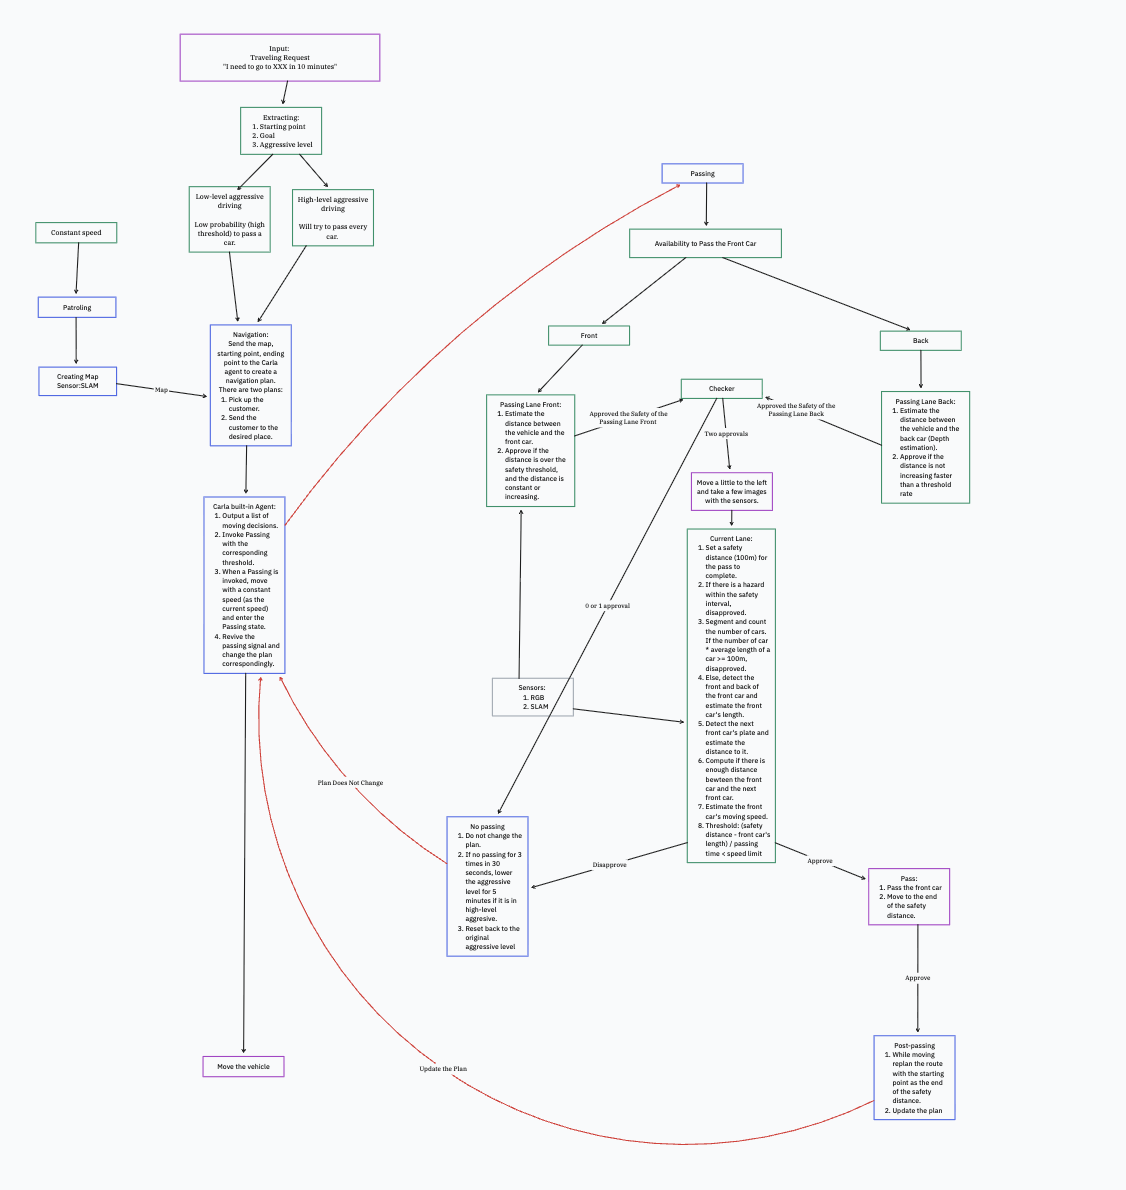
\includegraphics[height=0.78\textheight, width=\linewidth, keepaspectratio]{passing-diagram.png}
\end{center}
\end{frame}

\begin{frame}{Implemented Prototype Loop}
\begin{center}
\small
\begin{tabular}{c}
\texttt{ScenarioSpec} \\
$\downarrow$ \\
Request/Urgency Interpreter \\
$\downarrow$ \\
Perception/Map State Estimate \\
$\downarrow$ \\
Passing Agent: \texttt{pass / wait / replan} \\
$\downarrow$ \\
Safety Checker \\
$\downarrow$ \\
Execution Backend \\
$\downarrow$ \\
Evaluator: metrics + trace + failure type
\end{tabular}
\end{center}

\vspace{10pt}
\begin{center}
\textbf{Same interfaces will be reused for CARLA.}
\end{center}
\end{frame}

\begin{frame}{Scenario Representation}
\begin{itemize}
\item Each generated case is a structured object, not a one-off script.
\end{itemize}

\vspace{8pt}
\begin{center}
\small
\texttt{
\{request, route, ego, lead, rear, oncoming, occlusion, weather, sensor\}
}
\end{center}

\vspace{10pt}

\begin{itemize}
\item This lets us control:
\begin{itemize}
\item deadlines,
\item lead vehicle speed,
\item rear traffic,
\item oncoming gap,
\item visibility,
\item weather and sensor mode.
\end{itemize}
\end{itemize}
\end{frame}

\begin{frame}{Passing Decision}
\begin{itemize}
\item At each timestep, the agent estimates:
\begin{itemize}
\item front distance,
\item rear distance,
\item oncoming distance,
\item visibility,
\item urgency and delay cost.
\end{itemize}

\pause

\item Policy proposes:
\begin{center}
\Large
\texttt{pass} \quad \texttt{wait} \quad \texttt{replan}
\end{center}

\pause

\item Safety checker can reject unsafe pass proposals.
\end{itemize}
\end{frame}

\begin{frame}{Safety Constraint}
\begin{center}
\Large
\[
d_{\mathrm{gap}} >
v_{\mathrm{ego}}t_{\mathrm{pass}}
+\frac{1}{2}a_{\mathrm{ego}}t_{\mathrm{pass}}^2+\Delta
\]
\end{center}

\vspace{8pt}

\begin{itemize}
\item Urgency can increase willingness to consider passing.
\item It cannot override:
\begin{itemize}
\item low TTC,
\item unsafe rear traffic,
\item poor visibility,
\item insufficient oncoming gap.
\end{itemize}
\end{itemize}
\end{frame}

\begin{frame}{Policies Compared}
\begin{itemize}
\item \textbf{No-pass baseline}
\begin{itemize}
\item never passes,
\item exposes over-conservative delay.
\end{itemize}

\pause

\item \textbf{Aggressive baseline}
\begin{itemize}
\item pursues progress,
\item exposes unsafe passing.
\end{itemize}

\pause

\item \textbf{AutoPass}
\begin{itemize}
\item urgency-aware,
\item attempts selected passes,
\item safety checker rejects risky proposals.
\end{itemize}
\end{itemize}
\end{frame}

\begin{frame}{Initial Local Results: 50 Scenarios}
\begin{center}
\small
\begin{tabular}{lrrrr}
\toprule
Policy & Failures & Avg. time (s) & Pass attempts & Unsafe passes \\
\midrule
No-pass & 16/50 & 96.58 & 0 & 0 \\
AutoPass & 13/50 & 90.16 & 19 & 0 \\
Aggressive & 41/50 & 60.08 & 154 & 134 \\
\bottomrule
\end{tabular}
\end{center}

\vspace{10pt}

\begin{itemize}
\item Aggressive is fastest but unsafe.
\item No-pass is safe but slow.
\item AutoPass is the intended middle behavior.
\end{itemize}
\end{frame}

\begin{frame}{Failure Type Breakdown}
\begin{center}
\small
\begin{tabular}{lrrrr}
\toprule
Policy & None & Delay & Missed safe pass & Unsafe pass \\
\midrule
No-pass & 34 & 16 & 0 & 0 \\
AutoPass & 37 & 11 & 2 & 0 \\
Aggressive & 9 & 2 & 0 & 39 \\
\bottomrule
\end{tabular}
\end{center}

\vspace{10pt}

\begin{itemize}
\item AutoPass reduces delay failures relative to no-pass.
\item AutoPass avoids unsafe passes in this local evaluation.
\item Aggressive fails mostly through unsafe passing.
\end{itemize}
\end{frame}

\begin{frame}{What We Learned From the Prototype}
\begin{itemize}
\item The architecture runs end-to-end.
\item The traces are useful for debugging and explaining decisions.
\item Generated scenarios already expose meaningful behavior:
\begin{itemize}
\item conservative delay,
\item unsafe passing,
\item missed safe opportunities.
\end{itemize}

\pause

\item We also fixed two local backend issues:
\begin{itemize}
\item lane-aware collision logic,
\item safe car-following for wait/replan actions.
\end{itemize}
\end{itemize}
\end{frame}

\begin{frame}{Honest Limitation}
\begin{center}
\Large
\textbf{Current results are local prototype results, not full CARLA results.}
\end{center}

\vspace{14pt}

\begin{itemize}
\item Local backend uses lightweight kinematics.
\item It validates interfaces and the closed-loop evaluation logic.
\item Next step is replacing world state and execution with CARLA:
\begin{itemize}
\item actor spawning,
\item sensors,
\item map routes,
\item vehicle controls.
\end{itemize}
\end{itemize}
\end{frame}

\begin{frame}{Week 2 Plan: Minimal CARLA Integration}
\begin{itemize}
\item Take one \texttt{ScenarioSpec}.
\item Spawn:
\begin{itemize}
\item ego vehicle,
\item slow lead vehicle,
\item rear vehicle,
\item oncoming vehicle.
\end{itemize}

\pause

\item Set route, weather, and sensor configuration.
\item Run one pass/wait/replan rollout.
\item Save the same trace and metrics format.
\end{itemize}

\vspace{8pt}
\begin{center}
\textbf{Goal: one working CARLA-backed passing scenario.}
\end{center}
\end{frame}

\begin{frame}{Team Responsibilities}
\begin{itemize}
\item \textbf{Rohan:} integration, evaluation, plots, report, demo script.
\item \textbf{Xinwei:} passing logic, safety checker, decision-diagram alignment.
\item \textbf{Pranav:} CARLA actor spawning, routes, weather, sensors.
\item \textbf{Rathang:} perception/map tools, baselines, metrics, trace examples.
\end{itemize}

\vspace{10pt}
\begin{center}
\textbf{Shared contract: \texttt{ScenarioSpec} in, \texttt{PassState}/metrics out.}
\end{center}
\end{frame}

\begin{frame}{What We Want Feedback On}
\begin{itemize}
\item Is the current simulator-independent prototype a reasonable Week 1 checkpoint?
\item Is the CARLA integration plan scoped correctly?
\item Should we prioritize:
\begin{itemize}
\item stronger scenario generation,
\item more realistic CARLA execution,
\item or RGB/depth perception modules?
\end{itemize}
\item Are the failure types appropriate for the final report?
\end{itemize}
\end{frame}

\begin{frame}{Closing}
\begin{center}
\Large
\textbf{AutoPass-Gen turns passing into a stress-test problem.}\\[10pt]
\textbf{The goal is not just to drive, but to find the boundary where driving policies fail.}
\end{center}
\end{frame}

\end{document}